\section{Metodologia}

Este capítulo apresenta os procedimentos metodológicos adotados para o desenvolvimento deste trabalho e que será usado para o treinamento da regressão simbólica. Nele são descritos a implementação inicial do modelo de Black--Scholes acompanhada de gráficos preliminares com parâmetros previamente configurados e a avaliação do comportamento inicial das gregas. Também inclui a criação do conjunto de dados,
a configuração da regressão simbólica e os critérios utilizados para a
avaliação dos resultados.

\subsection{Implementação analítica do Modelo de Black--Scholes e das Gregas}
A implementação computacional do modelo de Black--Scholes foi realizada em
Python. Foram desenvolvidas funções específicas para o cálculo do preço de
opções europeias de compra (\textit{call}) e de venda (\textit{put}).

Para a opção de compra, foram inicialmente calculados os termos auxiliares
$d_1$ e $d_2$, definidos por
\begin{equation}
d_1 =
\frac{
\ln\left(\frac{S}{K}\right)
+
\left(r+\frac{\sigma^2}{2}\right)T
}{
\sigma\sqrt{T}
},
\end{equation}

\begin{equation}
d_2 = d_1 - \sigma\sqrt{T}.
\end{equation}

Em seguida, o preço da opção de compra foi calculado por
\begin{equation}
C =
S\Phi(d_1)
-
Ke^{-rT}\Phi(d_2).
\end{equation}
A partir da formulação analítica apresentada, implementou-se uma função em Python para calcular o preço de opções europeias de compra. A implementação utiliza a função de distribuição acumulada da normal padrão, disponibilizada pela biblioteca scipy.stats, e recebe como argumentos os parâmetros de precificação. Essa função foi utilizada posteriormente na geração dos valores de referência empregados nos experimentos de regressão simbólica.


\Needspace{17\baselineskip}

\begin{lstlisting}[
    language=Python,
    caption={Implementação do modelo de Black--Scholes para opções de compra europeia},
    label={lst:black_scholes_call}
]
import numpy as np
from scipy.stats import norm

def black_scholes_call_EU(S, K, tau, R, sigma):
    if tau <= 0:
        return max(S - K, 0)

    d1 = (np.log(S/ K) + (R + 0.5 * sigma**2) * tau) / (sigma *np.sqrt(tau))
    d2 = d1 - sigma* np.sqrt(tau)
    call_price = S * norm.cdf(d1) - K *np.exp(-R * tau) * norm.cdf(d2)
    return call_price
\end{lstlisting}
A implementação apresentada no Código 1 foi utilizada para gerar os preços teóricos das opções de compra, que posteriormente constituíram os valores de referência para o treinamento e a avaliação dos modelos de regressão simbólica.
Em que $S$ representa o preço atual do ativo subjacente, $K$ corresponde
ao preço de exercício da opção (\textit{strike price}), $r$ representa a
taxa de juros livre de risco e $\tau$  corresponde ao tempo restante até o
vencimento da opção. Além disso, $\Phi(\cdot)$ representa a função de
distribuição acumulada da distribuição normal padrão.

A função implementada também considera o caso em que o tempo restante até o
vencimento é igual a zero, o valor da opção corresponde diretamente ao seu \textit{payoff} \cite{brenndoerfer2025blackscholes}.

\begin{equation}
C_T = \max(S-K,0).
\end{equation}


Após a implementação das funções de precificação,
realizou-se uma análise gráfica exploratória com o
objetivo de verificar o comportamento das opções
europeias de compra e venda em função do preço
do ativo subjacente.

Nessa etapa preliminar, foram mantidos constantes
o preço de exercício $K=100$, o tempo restante
até o vencimento $\tau=1$ ano, a taxa livre
de risco $r=0{,}05$ e a volatilidade
$\sigma=0{,}20$, enquanto $S$ foi variado
entre 50 e 150.

Essa análise teve caráter exploratório,
destinando-se à verificação das propriedades
da implementação computacional, não sendo
utilizada no treinamento dos modelos de
regressão simbólica.

\begin{figure}[H]
    \centering
    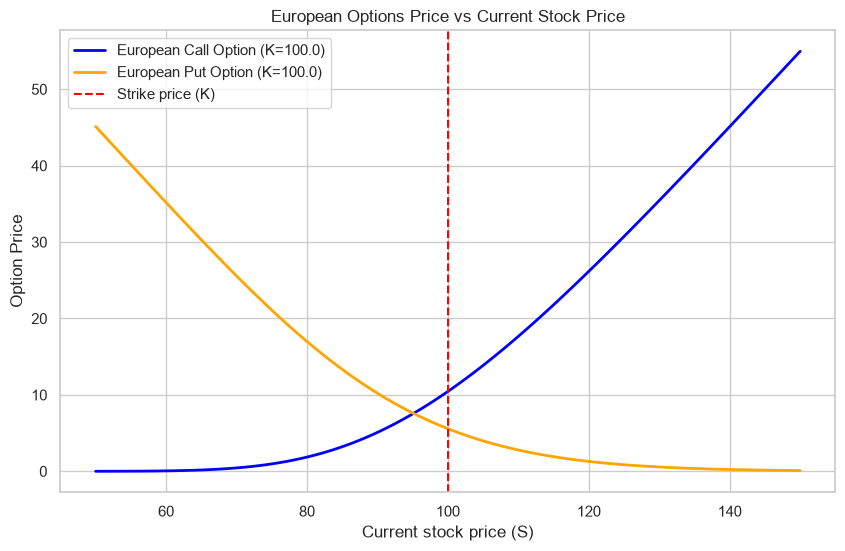
\includegraphics[width=0.8\textwidth]{Figs/bs_graph1.png}
    \caption{Comportamento dos preços das opções europeias de compra e venda
    em função do preço do ativo subjacente.}
    \label{fig:black_scholes_call_put}
    \small Elaborado pelo autor.
\end{figure}
É possível observar a convexidade do preço da opção de compra em relação ao
preço do ativo subjacente. Conforme discutido por Black e Scholes
\cite{blackscholes1973}, a curva que relaciona o valor da opção ao preço
do ativo apresenta curvatura positiva. No modelo de Black--Scholes, essa
propriedade pode ser expressa pela segunda derivada do preço da opção em
relação a $S$,

\begin{equation}
\frac{\partial^2 C}{\partial S^2} = \Gamma > 0.
\end{equation}
No gráfico obtido, esse comportamento pode ser observado pelo aumento
progressivo da inclinação da curva da opção à medida que $S$
aumenta. A relação entre o preço do ativo subjacente $S$ e o preço de exercício $K$
permite classificar a opção quanto ao seu \textit{moneyness}. Para uma opção
de compra (\textit{call}), quando $S<K$, a opção encontra-se
\textit{out of the money} (OTM); quando $S=K$, encontra-se
\textit{at the money} (ATM); e, quando $S>K$, encontra-se
\textit{in the money} (ITM).

Para uma opção de venda (\textit{put}), essa relação ocorre de forma inversa:
quando $S<K$, a opção está ITM; quando $S=K$, está ATM; e, quando $S>K$,
está OTM.

Após a implementação das funções de precificação das opções de compra e
venda, foram implementadas as principais gregas do modelo de
Black--Scholes: Delta, Gamma, Vega, Theta e Rho. Essas medidas representam
as sensibilidades do preço da opção em relação a diferentes parâmetros do
modelo.


Após a implementação das funções de precificação,
foram implementadas as principais Gregas do modelo
de Black--Scholes: Delta, Gamma, Vega, Theta e Rho.

As funções foram desenvolvidas a partir das
expressões analíticas apresentadas na
fundamentação teórica.

Para verificar graficamente o comportamento
dessas sensibilidades em relação ao preço
do ativo subjacente, utilizou-se a mesma
configuração de parâmetros adotada na
análise exploratória anterior, variando-se
$S$ entre 50 e 150.

Os resultados são apresentados na
Figura~\ref{fig:gregas}.

\begin{figure}[H]
    \centering
    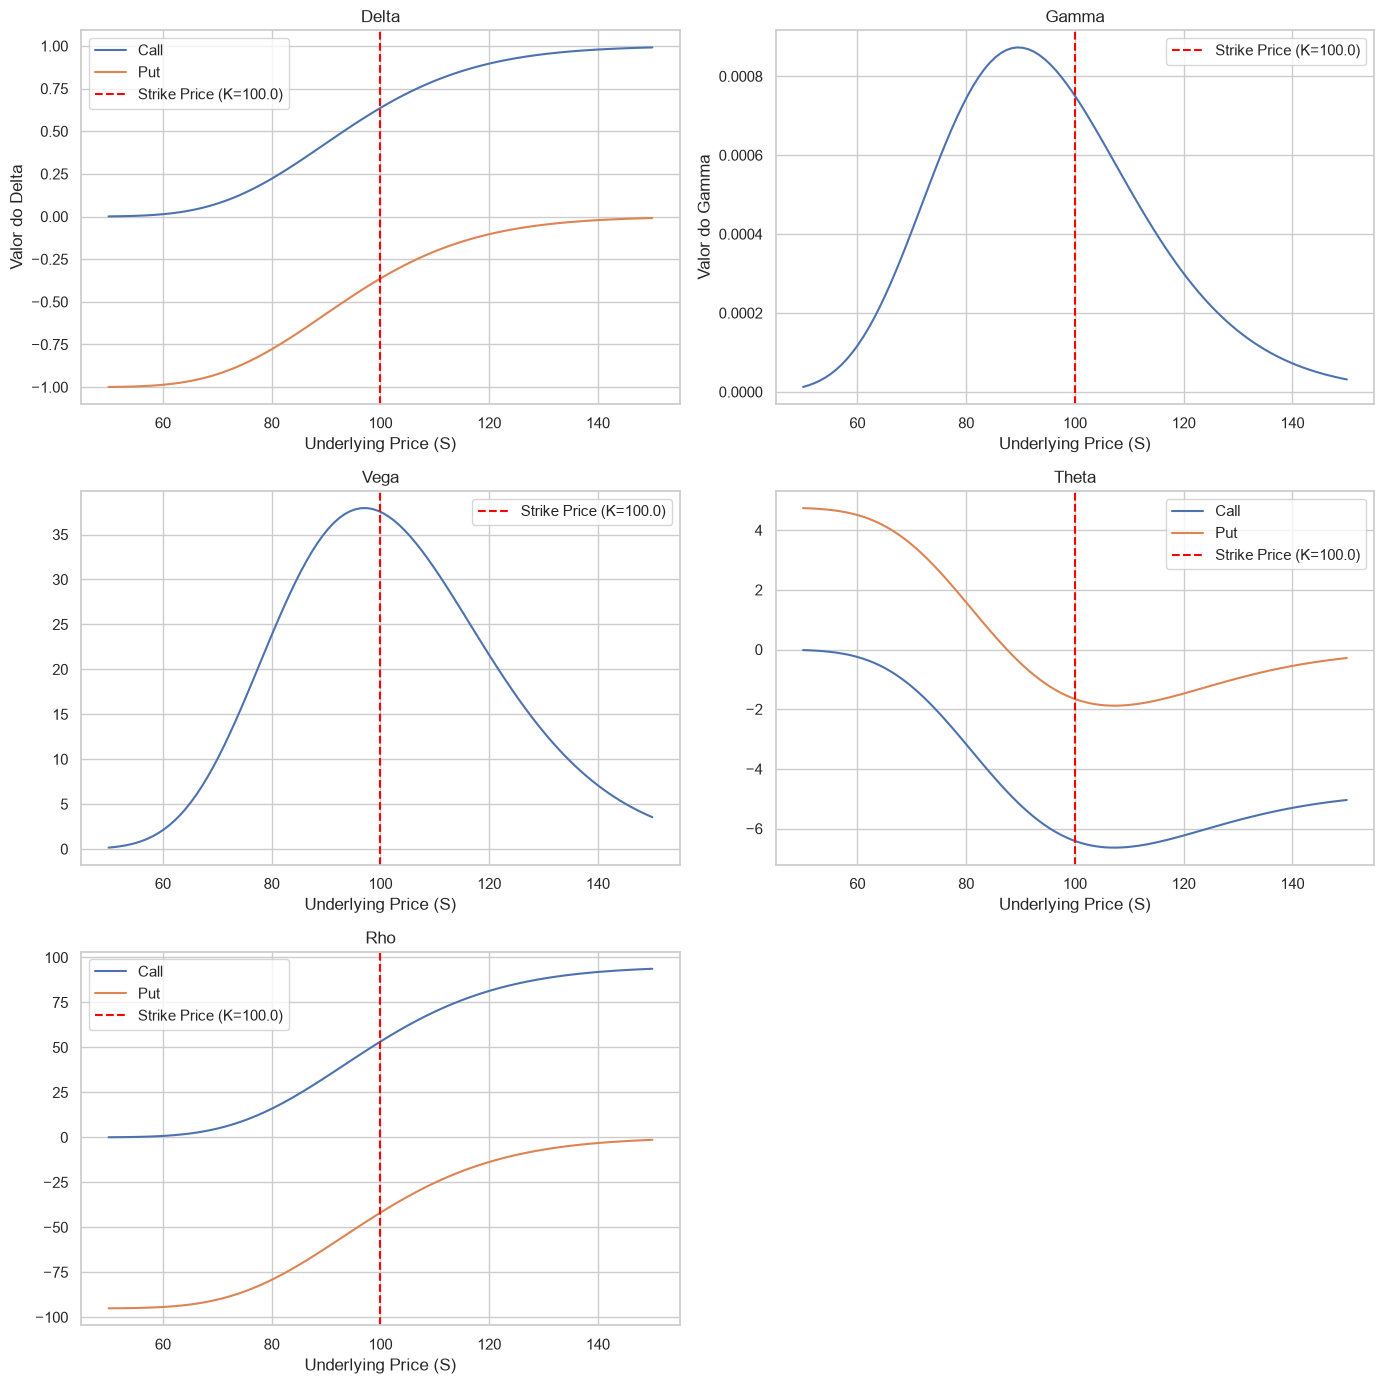
\includegraphics[width=\textwidth]{Figs/gregas.png}
    \caption{Comportamento das gregas em função do preço do ativo subjacente.}
    \label{fig:gregas}
    
    \small Elaborado pelo autor.
\end{figure}
\subsection{Análise Univariada de parâmetros}
Com o objetivo de investigar a capacidade da regressão simbólica de identificar relações matemáticas existentes no modelo de Black--Scholes, foi adotada uma abordagem univariada de cada parâmetro. Essa estratégia consiste em manter um parâmetro da precificação variando e os demais constantes, de modo a isolar cada contribuição para o comportamento do preço da opção. Essa abordagem permite analisar as expressões obtidas pelo PySR em condições controladas, reduzindo a influência simultânea das demais variáveis. Além disso, possibilita comparar as expressões
geradas com as aproximações analíticas apresentadas
na fundamentação teórica, em especial as
expansões de Taylor e de Puiseux. Em todos os casos,
o preço de exercício foi mantido fixo em $K=100$.
Nos experimentos em que $S$ permaneceu constante,
adotou-se $S=100$; nos demais, os parâmetros
fixos foram $r=0{,}05$, $\sigma=0{,}20$ e
$\tau=180/252$, conforme a variável investigada. Nesta etapa, os valores utilizados como referência foram
calculados diretamente pela solução analítica
de Black--Scholes, já implementada e detalhada anteriormente. Para cada experimento, os dados foram organizados
em conjuntos de treinamento e teste, utilizados,
respectivamente, para o ajuste das expressões
simbólicas e para a avaliação de sua capacidade
preditiva. As expressões obtidas foram analisadas
considerando o erro de aproximação, a complexidade
simbólica e a correspondência com as propriedades
matemáticas do modelo de Black--Scholes.

Essa abordagem estabelece uma referência inicial
para a investigação da regressão simbólica,
permitindo distinguir a recuperação de estruturas
matemáticas individuais da aproximação de relações
mais complexas entre múltiplas variáveis.
\subsubsection{Configuração dos Experimentos Univariados}
\subsubsection*{Variação do tempo até o vencimento ($\tau$)}

O primeiro experimento univariado investigou a
dependência do preço de uma opção europeia de compra
em relação ao tempo restante até o vencimento,
$\tau$. Nesse experimento, apenas $\tau$ foi
considerado variável independente, enquanto os
demais parâmetros do modelo de Black--Scholes
permaneceram constantes.

Foram adotados o preço do ativo subjacente
$S=100$, o preço de exercício $K=100$,
a taxa livre de risco $r=0{,}05$ e a
volatilidade $\sigma=0{,}20$.

Para construir o conjunto de dados, foram
considerados 180 valores do tempo restante
até o vencimento, correspondentes aos prazos
de 1 a 180 dias úteis. Esses valores foram
convertidos para anos, utilizando a convenção
de 252 dias úteis, conforme:

\begin{equation}
    \tau_i = \frac{d_i}{252},
    \qquad d_i \in \{1,2,\ldots,180\}.
\end{equation}

Dessa forma, o experimento compreendeu o
intervalo de $\tau \in [1/252,180/252]$.
Para cada valor de $\tau_i$, o preço
teórico da opção foi calculado diretamente
pela formulação analítica de Black--Scholes,
constituindo a variável-alvo do treinamento.

O conjunto resultante foi dividido em
144 observações para treinamento (80\%)
e 36 para teste (20\%). A separação foi
realizada de maneira determinística,
reservando os maiores valores de $\tau$
para treinamento e os menores para teste.

Além dos preços calculados diretamente pela
formulação de Black--Scholes, foram determinados
os coeficientes teóricos da expansão assintótica
em função de $\tau$, considerando a condição \textit{at-the-money} ($S=K$). Para isso, implementou-se uma função em Python
que calcula os coeficientes associados aos
termos $\tau^{1/2}$, $\tau$, $\tau^{3/2}$
e $\tau^2$, conforme a expansão de Puiseux
apresentada na fundamentação teórica. Esses coeficientes foram calculados
independentemente do treinamento do PySR,
sendo utilizados posteriormente como
referência analítica para avaliar a
correspondência entre as expressões obtidas
pela regressão simbólica e a estrutura
assintótica do modelo de Black--Scholes.
A implementação recebe como parâmetros os valores
de $S$, $K$, $r$ e $\sigma$, retornando os
coeficientes associados aos termos
$\tau^{1/2}$, $\tau$, $\tau^{3/2}$ e $\tau^2$,
respectivamente. Resumindamente, em forma de tabela, tem-se:

A Tabela~\ref{tab:parametros_tau} sintetiza os parâmetros
utilizados no primeiro experimento univariado,
destacando a variável investigada e os valores
mantidos constantes.


\begin{table}[htbp]
    \centering
    \caption{Configuração dos parâmetros do experimento univariado com $\tau$.}
    \label{tab:parametros_tau}

    \begin{tabular}{lcc}
        \hline
        \textbf{Parâmetro} &
        \textbf{Condição} &
        \textbf{Valor utilizado} \\
        \hline
        Preço do ativo ($S$) & Constante & $100$ \\
        Preço de exercício ($K$) & Constante & $100$ \\
        Taxa livre de risco ($r$) & Constante & $0{,}05$ \\
        Volatilidade ($\sigma$) & Constante & $0{,}20$ \\
        Tempo até o vencimento ($\tau$) &
        Variável & $[1/252,\;180/252]$ ano \\
        \hline
        Total de observações & --- & $180$ \\
        Treinamento & 144 observações &
        $\tau \in [37/252,\;180/252]$ \\
        Teste & 36 observações &
        $\tau \in [1/252,\;36/252]$ \\
        \hline
    \end{tabular}

    \vspace{0.2cm}
    {\footnotesize Fonte: Elaboração própria.\par}
\end{table}


A precisão das expressões identificadas pelo PySR
foi avaliada por meio do erro absoluto médio
(MAE), do erro quadrático médio (MSE) e da raiz
do erro quadrático médio (RMSE).

Essas métricas foram calculadas sobre os conjuntos
de teste, considerando como referência os preços
obtidos pela formulação analítica de Black--Scholes. Além da avaliação preditiva, foram consideradas
a complexidade simbólica das expressões e sua
correspondência com as propriedades matemáticas
do modelo de referência, incluindo os coeficientes
das expansões de Taylor e de Puiseux.

\subsubsection*{Variação da taxa de juros ($r$)}
O segundo experimento univariado investigou a dependência
do preço de uma opção europeia de compra em relação à taxa
livre de risco, $r$. Nesse experimento, apenas a taxa de
juros foi considerada variável independente, enquanto
os demais parâmetros do modelo de Black--Scholes
permaneceram constantes. Foram adotados o preço do ativo subjacente $S=100$,
o preço de exercício $K=100$, a volatilidade
$\sigma=0{,}20$ e o tempo restante até o vencimento
$\tau=180/252$ ano. Para a construção do conjunto de dados, foram
considerados 91 valores da taxa livre de risco,
distribuídos uniformemente no intervalo de
$0{,}01$ a $0{,}10$, com incrementos de $0{,}001$.
Assim, os valores da variável independente
foram definidos por:

\begin{equation}
r_i = 0{,}01 + 0{,}001i,
\qquad i \in \{0,1,\ldots,90\}.
\end{equation}

Essa separação determinística permitiu avaliar
a capacidade de extrapolação das expressões
simbólicas para taxas superiores às utilizadas
durante o treinamento.

Além da avaliação dos preços calculados pelo
PySR, foram determinados os coeficientes
teóricos da expansão de Taylor de segunda
ordem da função de Black--Scholes em relação
à taxa livre de risco, considerando como
ponto de expansão $r_0=0$.

A aproximação analítica foi expressa por:

\begin{equation}
C_{BS}(r) =
a_0 + a_1r + a_2r^2 + \mathcal{O}(r^3),
\end{equation}

em que $a_0$ corresponde ao preço teórico
da opção em $r=0$, $a_1$ representa a
primeira derivada do preço em relação à
taxa livre de risco, associada à sensibilidade
Rho, e $a_2$ corresponde à metade da
segunda derivada em relação a $r$. Ressalta-se que os preços utilizados no treinamento
foram obtidos pela formulação analítica exata
de Black--Scholes, enquanto a expansão de Taylor
foi empregada exclusivamente na comparação
das propriedades matemáticas das expressões
identificadas. A tabela ~\ref{tab:parametros_r} abaixo mostra um resumo dos parâmetros.


\begin{table}[htbp]
    \centering
    \caption{Configuração do experimento univariado
    com a taxa livre de risco ($r$).}
    \label{tab:parametros_r}

    \begin{tabular}{lcc}
        \hline
        \textbf{Parâmetro} &
        \textbf{Condição} &
        \textbf{Valor utilizado} \\
        \hline
        Preço do ativo ($S$) & Constante & $100$ \\
        Preço de exercício ($K$) & Constante & $100$ \\
        Volatilidade ($\sigma$) & Constante & $0{,}20$ \\
        Tempo até o vencimento ($\tau$) &
        Constante & $180/252$ ano \\
        Taxa livre de risco ($r$) &
        Variável & $[0{,}01;\,0{,}10]$ \\
        Incremento de $r$ & --- & $0{,}001$ \\
        \hline
        Total de observações & --- & $91$ \\
        Treinamento & 71 observações &
        $r \in [0{,}01;\,0{,}08]$ \\
        Teste & 20 observações &
        $r \in [0{,}081;\,0{,}10]$ \\
        \hline
    \end{tabular}

    \vspace{0.2cm}
    {\footnotesize Fonte: Elaboração própria.\par}
\end{table}

\subsubsection*{Variação da volatilidade ($\sigma$)}
O terceiro experimento univariado teve como objetivo
investigar a capacidade da regressão simbólica de
aproximar a relação entre a volatilidade e o preço
de uma opção europeia de compra, mantendo constantes
os demais parâmetros do modelo de Black--Scholes. Foram adotados $S=K=100$, taxa livre de risco
$r=0{,}05$ e tempo restante até o vencimento
$\tau=180/252$ ano. Para a construção do conjunto de dados, foram
considerados 31 valores de volatilidade,
igualmente espaçados entre $0{,}10$ e $0{,}40$,
com incrementos de $0{,}01$. Para cada valor
de $\sigma$, o preço teórico da opção foi
calculado diretamente pela formulação analítica
de Black--Scholes, constituindo a variável-alvo
do experimento.

O conjunto de dados foi ordenado de maneira
crescente em relação à volatilidade e dividido
em 24 observações para treinamento e 7 para
teste. O treinamento compreendeu valores de
$\sigma$ entre $0{,}10$ e $0{,}33$, enquanto
o conjunto de teste contemplou valores entre
$0{,}34$ e $0{,}40$. Essa divisão determinística
permitiu avaliar a capacidade de extrapolação
das expressões identificadas pelo PySR para
volatilidades superiores às observadas durante
o treinamento. Além da avaliação da precisão dos preços
estimados, foram determinados os coeficientes
teóricos da expansão de Taylor de segunda
ordem da função de Black--Scholes em relação
à volatilidade, considerando como ponto de
expansão $\sigma_0=0{,}20$.

A aproximação analítica foi expressa por:

\begin{equation}
\begin{aligned}
C_{BS}(\sigma) \approx {}&
a_0+a_1(\sigma-\sigma_0)\\
&+a_2(\sigma-\sigma_0)^2,
\end{aligned}
\end{equation}

em que $a_0$ corresponde ao preço da opção
no ponto de expansão, $a_1$ representa
a primeira derivada em relação à volatilidade
(Vega) e $a_2$ corresponde à metade da
segunda derivada em relação à volatilidade
(Vomma).
Para os parâmetros fixados, os coeficientes
teóricos calculados foram:

\begin{equation}
\begin{aligned}
C_{BS}(\sigma) \approx {}&
8{,}518175855\\
&+32{,}273470128(\sigma-0{,}20)\\
&+3{,}025637825(\sigma-0{,}20)^2.
\end{aligned}
\end{equation}

Esses coeficientes foram obtidos
independentemente do treinamento do PySR,
por meio de uma função implementada em Python.
A expansão foi utilizada como referência
para investigar se as expressões simbólicas
identificadas reproduzem o comportamento
local da função de precificação, incluindo
sua sensibilidade e curvatura em relação
à volatilidade. A Tabela~\ref{tab:parametros_sigma} apresenta um resumo
dos parâmetros utilizados no experimento em que
a volatilidade ($\sigma$) é variável.


\begin{table}[htbp]
    \centering
    \caption{Configuração dos parâmetros do experimento univariado com $\sigma$.}
    \label{tab:parametros_sigma}

    \begin{tabular}{lcc}
        \hline
        \textbf{Parâmetro} &
        \textbf{Condição} &
        \textbf{Valor utilizado} \\
        \hline
        Preço do ativo ($S$) & Constante & $100$ \\
        Preço de exercício ($K$) & Constante & $100$ \\
        Taxa livre de risco ($r$) & Constante & $0{,}05$ \\
        Tempo até o vencimento ($\tau$) &
        Constante & $180/252$ ano \\
        Volatilidade ($\sigma$) &
        Variável & $[0{,}10;\,0{,}40]$ \\
        Incremento de $\sigma$ & --- & $0{,}01$ \\
        \hline
        Total de observações & --- & $31$ \\
        Treinamento & 24 observações &
        $\sigma \in [0{,}10;\,0{,}33]$ \\
        Teste & 7 observações &
        $\sigma \in [0{,}34;\,0{,}40]$ \\
        \hline
    \end{tabular}

    \vspace{0.2cm}
    {\footnotesize Fonte: Elaboração própria.\par}
\end{table}


% Impede que as tabelas dos experimentos ultrapassem esta subseção.
\FloatBarrier
\subsubsection*{Variação do preço do ativo ($S$)}
O experimento univariado com o preço do ativo subjacente  
teve como objetivo investigar a capacidade da regressão simbólzica de aproximar a função de precificação de Black--Scholes quando apenas a variável $S$ é modificada. Para isso, foram mantidos constantes o preço de exercício $K=100$, a taxa livre de risco $r=0{,}05$, a volatilidade $\sigma=0{,}20$ e o tempo restante até o vencimento $\tau=180/252$ ano.

O \textit{dataset} foi construído a partir de 91 valores igualmente espaçados de ($S$), compreendidos entre 70 e 130. Para cada observação, o preço teórico da opção europeia de compra foi calculado diretamente pela formulação analítica de Black-Scholes, constituindo a variável-alvo do treinamento. Os dados foram ordenados de maneira crescente e particionados deterministicamente em 71 observações de treinamento e 20 de teste, correspondentes, respectivamente, aos intervalos de aproximadamente 70 a 116,67 e de 117,33 a 130. Essa divisão foi adotada para avaliar a capacidade de extrapolação das expressões simbólicas para preços do ativo superiores aos utilizados durante o ajuste.
Como uma primeira rodade de testes, realizou-se o treinamento utilizando a configuração padrão estabelecida para os experimentos univariados, com 500 iterações, operadores binários de adição, subtração, multiplicação e divisão, e operadores unários exponencial, logaritmo, raiz quadrada e função erro (\textit{erf}). O tamanho máximo das expressões foi limitado a 35, utilizando-se o critério \texttt{model\_selection=best} para a seleção automática de uma expressão pelo PySR.

A investigação foi organizada em duas rodadas independentes de treinamento do PySR, diferenciadas pela configuração dos hiperparâmetros responsáveis pela exploração do espaço de busca simbólica. Em ambas, foram utilizados os mesmos conjuntos de treinamento e teste, mantendo-se ($S$) como a única variável independente.

Na primeira rodada de treinamento, adotou-se a configuração inicial estabelecida para os experimentos univariados, com 500 iterações, operadores binários de adição, subtração, multiplicação e divisão, além dos operadores unários exponencial, logaritmo, raiz quadrada e função erro (erf). O tamanho máximo das expressões foi limitado a 35, utilizando-se o critério \texttt{model\_selection="best"} para a seleção automática de uma expressão pelo PySR. Após o treinamento, as expressões preservadas pelo algoritmo foram avaliadas quanto à precisão preditiva nos conjuntos de treinamento e teste, considerando também sua complexidade simbólica.

Na segunda rodada, realizou-se um novo treinamento independente, com uma configuração ampliada de hiperparâmetros, visando investigar a influência de uma busca evolutiva mais extensa sobre as expressões identificadas. Nessa execução, o número de iterações foi aumentado para 1.200, com 24 populações e 40 indivíduos por população. Também foram definidos 500 ciclos evolutivos por iteração, tamanho máximo de expressão igual a 40 e profundidade máxima igual a 12. Os operadores matemáticos e o critério de seleção foram mantidos em relação à primeira rodada, sendo utilizada a semente aleatória \texttt{random\_state=42}. Adicionalmente, foi realizada uma análise da correspondência entre as expressões simbólicas e as propriedades analíticas do modelo de Black-Scholes. Para isso, considerou-se a expansão teórica de Taylor de segunda ordem em relação a $S$, em torno do ponto ($S_0=100$). Para cada expressão selecionada para análise, foram calculados seu valor, sua primeira derivada e a segunda derivada no ponto de expansão, permitindo a comparação com o preço teórico da opção, Delta e metade de Gamma.

De maneira complementar, as derivadas das expressões foram avaliadas em uma malha de 301 pontos no intervalo de ($S=70$) a ($S=130$). Esse procedimento permitiu investigar a correspondência com as sensibilidades analíticas de Black-Scholes e verificar a preservação de propriedades matemáticas, como monotonicidade, limites de Delta e convexidade.

Para a avaliação das expressões, foram considerados o erro absoluto médio (MAE), o erro quadrático médio (MSE), a raiz do erro quadrático médio (RMSE) e a complexidade simbólica ,ou seja seu sentido matemático e financeiro , esta análise de desempenho considerou tanto a interpretabilidade no domínio do problema, atestada pelo comportamento das Gregas, quanto a eficiência matemática. Além da expressão selecionada automaticamente pelo algoritmo, foram examinadas outras expressões preservadas pelo PySR, permitindo investigar diferentes compromissos entre precisão numérica e sentido financeiro e matemático. Abaixo uma tabela resumindo quais fora os hiper parâmetros usados nos experimentos.


\begin{table}[htbp]
    \centering
    \caption{Configurações dos hiperparâmetros duas execuções do PySR
    para a variação do preço do ativo subjacente.}
    \label{tab:configuracoes_pysr_S}

    \begin{tabular}{lcc}
        \hline
        \textbf{Hiperparâmetro} &
        \textbf{Inicial} &
        \textbf{Ampliada} \\
        \hline
        \texttt{niterations} & 500 & 1200 \\
        \texttt{populations} & 31 & 24 \\
        \texttt{population\_size} & 27 & 40 \\
        \texttt{ncycles\_per\_iteration} & 380 & 500 \\
        \texttt{maxsize} & 35 & 40 \\
        \texttt{maxdepth} & \texttt{None} & 12 \\
        \texttt{model\_selection} & best & best \\
        \texttt{random\_state} & \texttt{None} & 42 \\
        \hline
    \end{tabular}

    \vspace{0.2cm}
    {\footnotesize Fonte: Elaboração própria.\par}
\end{table}
A seguir, a Tabela~\ref{tab:parametros_S} resume a dinâmica desta rodada de testes em relação ao preço do ativo $S$.
\begin{table}[H]
    \centering
    \caption{Configuração dos parâmetros do experimento univariado com $S$.}
    \label{tab:parametros_S}
    
    \begin{tabular}{lcc}
        \hline
        \textbf{Parâmetro} & \textbf{Condição} & \textbf{Valor utilizado} \\
        \hline
        Preço do ativo ($S$) & Variável & $[70;130]$ \\
        Preço de exercício ($K$) & Constante & 100 \\
        Taxa livre de risco ($r$) & Constante & 0,05 \\
        Tempo até o vencimento ($\tau$) & Constante & $180/252$ ano \\
        Volatilidade ($\sigma$) & Constante & 0,20 \\
        Incremento de $S$ & --- & $2/3 \approx 0,6667$ \\
        \hline
        \textbf{Total de observações} & --- & \textbf{91} \\
        \hline
        Treinamento & 71 observações & $S \in [70;116,67]$ \\
        Teste & 20 observações & $S \in [117,33;130]$ \\
        \hline
    \end{tabular}

    \vspace{0.2cm}
    {\footnotesize Fonte: Elaboração própria.\par}
\end{table}

\subsection{Configuração da Regressão Simbólica}

\subsection{Procedimento Experimental}

\subsection{Métricas de Avaliação}
